% !TEX root = 15cvpr.tex
\section{Introduction}

\begin{figure}[t]
\begin{center}
    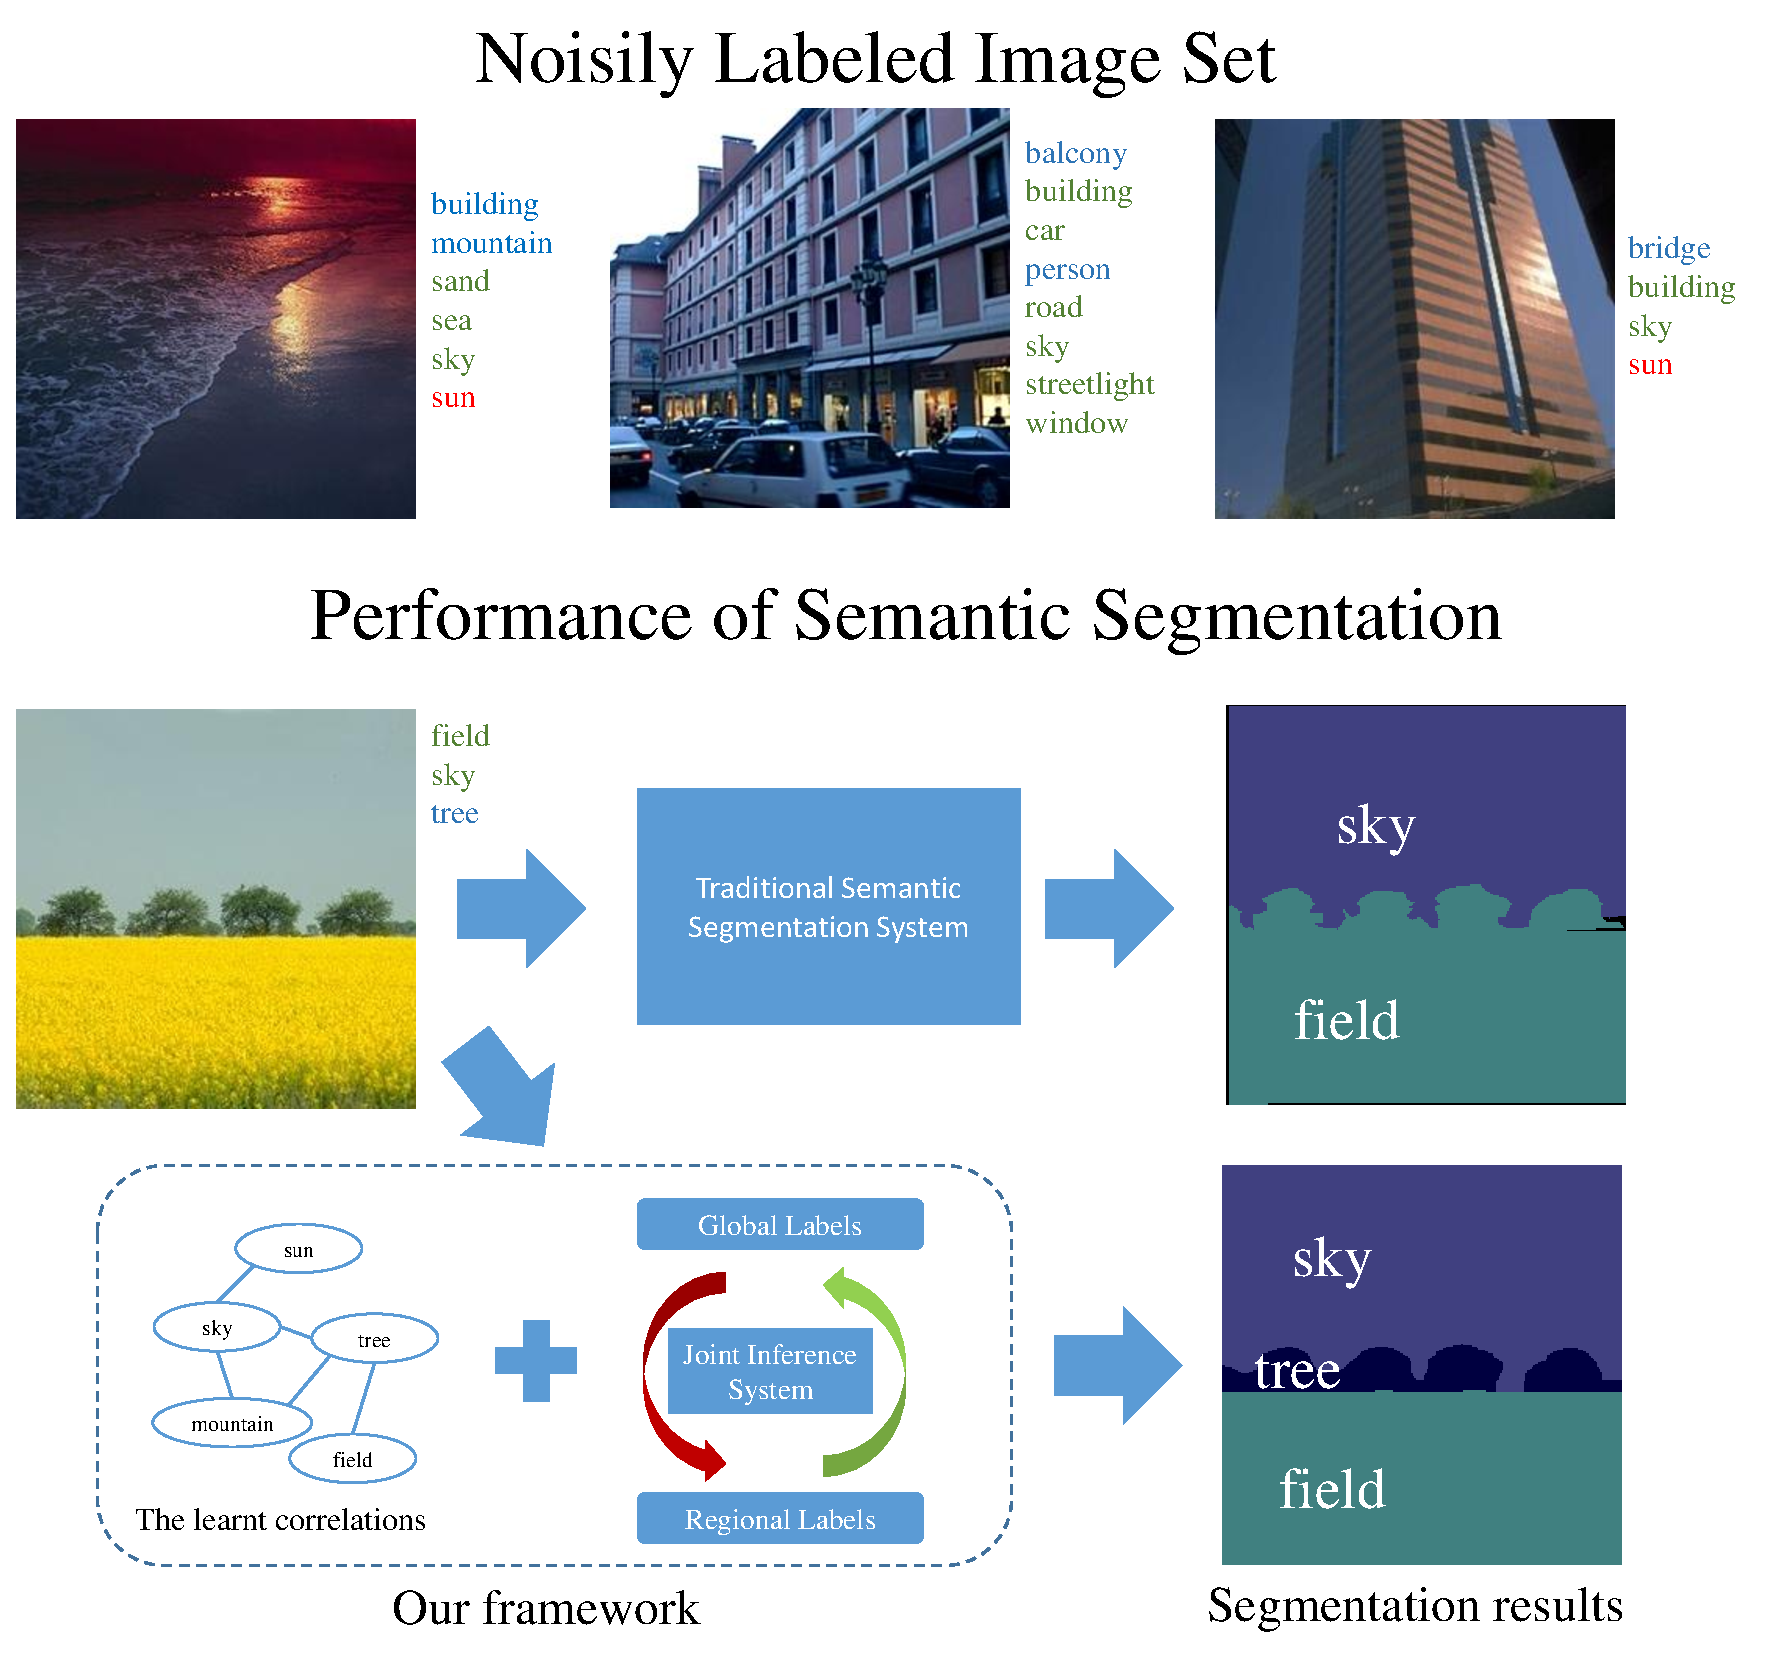
\includegraphics[width=1\linewidth]{fig_noisyparsing.pdf}
\end{center}
    \caption{In this paper, weakly supervised settings are summarized as two aspects: on the one hand, only source of annotation are image-level labels encoding which categories are present in the image. On the other hand, noisy annotations in real-world setting further relax the constraints, labels must be precise and complete. Given a training set of real-world images and its associated labels where label may be precise (green), incorrect (red) or missing (blue), we learn a model that segments and recognizes visual concept in new images. Best viewed in color.}
\label{fig:noisyparsing}
\end{figure}

Semantic segmentation, an attractive but challenging task in computer vision community, is an efficient way to handle an explosive growth in the volume of real-world images. Aiming to assign each pixel to one of predefined semantic categories, machine learning methods are utilized to learn classifier from labeled training images. Most state-of-the-art approaches heavily rely on extensive guidance in training, using a sufficiently huge amount of annotated samples, while the truth is only a subset of large-scale image dataset can be manually labeled, \textcolor{red}{due to its time-consuming and labor-intensive}. Recent works have begun to address the semantic segmentation problem under the weakly supervised settings, where each training image is annotated by image-level labels specifying which classes are present but no pixel-level annotation is given \cite{verbeek2007region,vezhnevets2010towards,vezhnevets2011weakly,vezhnevets2012weakly,xu2014tell,zhang2013sparse,zhang2013probabilistic}. With the prevalence of photo sharing websites and collaborative image tagging system, such as Flickr, which host vast of digital images with user provided tags, such weakly supervised methods are more flexible in real-world applications since the image-level annotated images are much easier to obtain.

Inspired by these works, we focus on the problem of weakly supervised semantic segmentation in real-world settings, which further relaxes the prerequisites for annotations (\eg labels must be precise and complete). It is worth noting that the annotations of collaboratively-tagged images may not be clean (incorrect or incomplete) in practice, but such noisy annotation has been ignored in recent work. It is not a realistic assumption in many real-world settings because collecting large-scale images with clean labels is still a labor-intensive task. Figure \ref{fig:noisyparsing} illustrates a set of representative real-world images and its associated tags. We can observe that only limited tags accurately describe the visual content of the image, while other tags are imprecise. Moreover, some important tags, which are highly associated with the image, are missing.

In this paper, We present a weakly supervised method that, for the first time, overcomes the challenge posed by noisy annotations, simultaneously achieves results competitive with fully supervised methods. The proposed method takes a novel framework that tries to integrate various contextual relations in a single framework for weakly supervised semantic segmentation in real-world settings, where only source of annotation are image-level labels encoding which categories are present in the image, and worse, the annotation can be noisy. The connections between high-level semantic concepts and low-level visual appearance are mined at both image-level and super-pixel level. The associations among semantic labels are captured by two aspects, inter-label co-occurrence statistics as well as discriminative regions overlap of concepts pairs. The label consistency between image-level and pixel-level is utilized for noisy annotation refinement by a joint inference with alternating procedure. These latent associations are significantly leveraged to advance segmentation performance even in noisy real-world settings.

To illustrate both robustness and effectiveness of our method, we demonstrate experiment results on two challenging datasets, PASCAL VOC 2007 and SIFT-flow datasets,  which are representative of the hardness of annotation noise occurs in real-world images. Our method outperforms previous state-of-the-art approaches on standard datasets, demonstrating that the image-level annotation, especially potential relationships, are more efficiently utilized by our method. Moreover, our approach perform comparable results even if segmenting real-world images without annotation, while only a limited subset of real-world image datasets with labor-intensive manually annotations is available.

The main contributions of this paper are summarized as follows:
\begin{enumerate}
  \item We propose a weakly supervised semantic segmentation framework in real-world settings, where only image-level labels are available, and worse, the annotations can be noisy. The experiment results on two real-world datasets demonstrate both effectiveness and robustness of our method, even in noisy annotation condition.
  \item We design a novel CRF model that jointly models various contextual relations in a single framework. It can be investigated from different perspectives: the associations between semantic concepts and visual appearance, co-relation among inter-class labels, label consistency between image-level and pixel-level.
  \item We propose a efficient method to model inter-label correlation that jointly captures inter-label co-occurrence statistics as well as discriminative regions overlap of concepts pairs. {\textcolor{red}{TBD:Details?}}
\end{enumerate}

\if

 We utilize a graphical model which incorporates image representations, visual appearance features and semantic topic distribution, and noisy image-level labels together with latent superpixel labels over the whole training set into one CRF model. A novel method is developed for achieving multi-label multi-instance image annotation, where image-level (bag-level) labels and region-level (instance-level) labels are both obtained. The associations between semantic concepts and visual features are mined both at the image level and at the region level. Inter-label correlations are captured by a co-occurrence matrix of concept pairs. The cross-level label coherence en- codes the consistency between the labels at the image level and the labels at the region level. The associations be- tween visual features and semantic concepts, the correlations among the multiple labels, and the cross-level label coherence are sufficiently leveraged to improve annotation performance.

We tackle semantic segmentation in real-world settings where only source of annotation are image-level labels encoding which categories are present in the image, and worse, the annotation can be noisy.

In the past few years, many different methods \cite{csurka2011efficient,gonfaus2010harmony,ladicky2009associative,nowozin2010parameter,shotton2008semantic,shotton2006textonboost,singh2013nonparametric,verbeek2007scene,yang2007multiple,yao2012describing} have been proposed for this task. Notwithstanding significant improvements they have achieved, most of them rely on full supervision: each pixel of the image for training is manually labeled by humans. The performance of these fully supervised methods heavily relies on a sufficiently huge amount of annotated samples, while the truth is only a subset of large-scale image dataset can be manual labeled, due to its time-consuming and labor-intensive. Therefore, these methods are inherently limited so that such system cannot be widely applied in practice.

Recently, a few works have been proposed to address the semantic segmentation problem under the weakly supervised settings, where each training image is annotated by image-level labels specifying which classes are present but no pixel-level annotation is given \cite{verbeek2007region,vezhnevets2010towards,vezhnevets2011weakly,vezhnevets2012weakly,xu2014tell,zhang2013sparse,zhang2013probabilistic}. Different from the traditional supervised semantic segmentation, such weakly supervised method is more flexible in real-world applications for the image-level annotated images are much easier to obtain. With the prevalence of photo sharing websites and collaborative image tagging system, such as Flickr, which host vast of digital images with user provided tags, this weakly supervised setting for image parsing become more and more feasible.

 Fortunately, owing to the collaborative image tagging system, \eg Flickr, we can easily obtain a large mount of manually labeled images provided by Internet users, though these image-level labels might be noisy (incorrect or incomplete). Therefore, the main challenge lies in how to utilize the noisily labeled images for semantic segmentation (see Figure \ref{fig:noisyparsing} for an illustration).


 Moreover, most existing semantic segmentation methods, either fully or weakly supervised, depend on a single choice of image partitioning (quantization). The precise quantization of an image is of significance, and it is less likely to obtain a common optimal quantization (partitioning) level suitable for every object. To overcome this problem, \cite{hoiem2005geometric,kohli2009robust,ladicky2009associative,nowozin2010parameter,russell2006using} used multiple segmentations of the image and achieved good performances by heuristic strategies or enforcing label consistency with higher order potential.

It is worth noting that the annotations of collaboratively-tagged images may not be accurate (incorrect or incomplete) in practice, but such noisily tagged annotation has been ignored in recent work. Moreover, there are some extra prerequisites (\eg labels must be precise and complete) for the initial image-level labels in existed weakly supervised semantic segmentation systems, while collecting such training images that satisfy all these constraints is still a labor-intensive task. Figure \ref{fig:noisyparsing} illustrates a set of representative real-world images and its associated tags. We can observe that only limited tags accurately describe the visual content of the image, while other tags are imprecise. Meanwhile, some important tags, which are highly associated with the image, are missing. Therefore, the main challenge lies in how to utilize the noisily labeled images for semantic segmentation.
\fi
